\section{Relationaler Datenbankentwurf}
\label{sec:abbildenRelational}

\textbf{Funktionale Abhängigkeiten (FD)}
\begin{items}
	\item In Relation \( R(X,Y) \) ist \( Y \) von \( X \) funktional abhängig (schreibe \( X \to Y \)), falls zu jedem \( X \)-Wert genau ein \( Y \)-Wert gehört \\*
	 (z.B. ISBN $\to$ Buchtitel, Inventarnr. oder Stadt $\to$ Bundesland)
	\item \( \leadsto \) ``\( X \) bestimmt \( Y \)''
	\item Festlegung der FDs a priori beim Schemaentwurf (enthält semantische Information für höhere Konsistenz), nicht hinterher aus dem Datenbestand
	\item Spezialfall \underline{Schlüssel} X für Relation R: $X \to R$ und X minimal
	\item \underline{Transitiv}: $X \to  Y  \to  Z \Rightarrow  X  \to Z$
	\item \( F \): Menge von FDs (\emph{funcional dependencies}), \( f \in F \) einzelne FD
	\item \( F \) impliziert \( f \): \( F \models f \)   $\qquad$  (bedeutet $SAT_R(F) \subseteq SAT_R(f)$)
	\item \underline{Hülle}: \( F_R^+ = \{ f \mid (f \text{ FD über} R) \wedge F \models f \} \)
	\item \underline{Reflexiv}: $X \to X$ (und $F \models X \to X$ für alle F, X)
	\item \underline{Akkumulativ}: $X \to YZ, Z \to VW \Rightarrow X \to YZV$
	\item \underline{Projektiv}: $X \to YZ \Rightarrow X \to Y$
	\item Äquivalente FD-Mengen (Überdeckungen): \( F \equiv G \) falls \( F^+ = G^+ \)
\end{items}

\textbf{RAP-Algorithmus für das Membership-Problem}
\begin{items}
	\item  Problem: Menge von FDs $F$. Gilt $X \to Y \in F^+$?
	\item Lösung in linearer Zeit:
	\begin{enumerate}
		\item $X^* :=  X$ (R-Regel)
		\item Erweitere $X^* := X^* \cup Y_1$ für $X_1 \to Y_1$ mit $X_1 \subseteq X^*$ bis $X^*$ stabil (A-Regel)
		\item Ist $Y \subseteq X^*$, gilt $X \to Y$ (P-Regel)
	\end{enumerate}
\end{items}

\textbf{Redundanzen - Anomalien}
\begin{items}
	\item Belegen unnötigen Speicherplatz
	\item Widersprüchliche oder fehlende Eingaben (\underline{Einfügeanomalie})
	\item Änderungen parallel in allen Vorkommen nötig (\underline{Updateanomalie})
	\item Informationen können beim Löschen anderer Inhalte mit verloren gehen (\underline{Löschanomalie})
\end{items}

\textbf{Abhängigkeitstreue}
\begin{items}
	\item Alle gegebenen Abhängigkeiten sind durch Schlüssel repräsentiert
	\item Genauer: Menge der Abhängigkeiten (FDs) äquivalent zur Menge der Schlüsselabhängigkeiten.
\end{items}

\textbf{Verbundtreue}
\begin{items}
	\item Originalrelationen können durch Verbund der Basisrelationen wiedergewonnen werden
	\item Kriterium für zwei Relationen:
	Dekomposition von X in $X_1$ und $X_2$ verbundtreu, wenn $X_1 \cap X_2 \to X_1$ oder $X_1 \cap X_2 \to X_2$
	\item Allgemeines Kriterium: 
	Wenn eine abhängigkeitstreue Dekomposition von R in $X_i$ einen Universalschlüssel erhält (also für ein $X_i$ gilt $X_i \to R$), so ist sie verbundtreu.
\end{items}

\textbf{Universalrelation}
\begin{items}
	\item \underline{Universalrelation} (von \( R_1, \dots, R_n \)): \( R = R_1 \bowtie \cdots \bowtie R_n \)
	\item \underline{Universalschlüssel}: Schlüssel der Universalrelation
	\item Beispiel: \( R_1, R_2, R_3 \):
	\begin{figure}[H]\centering\label{NonJoin}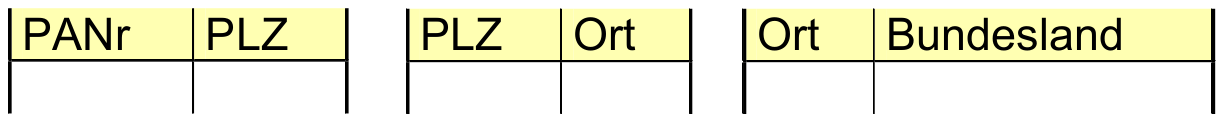
\includegraphics[width=0.33\textwidth]{NonJoin}\end{figure}
	\item \quad \( R_1 \bowtie R_2 \bowtie R_3 \):
	\begin{figure}[H]\centering\label{Join}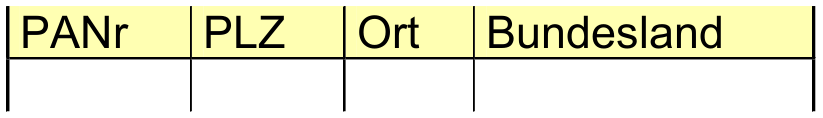
\includegraphics[width=0.33\textwidth]{Join}\end{figure}
\end{items}

\newpage

\textbf{Entwurfsziel}
\begin{items}
	\item Relationenschemata, (Fremd-)Schlüssel so wählen, dass
	\begin{enumeration}
		\item alle Anwendungsdaten aus Basisrelation hergeleitet werden können (\emph{Verbundtruee})
		\item nur semantisch sinnvolle und konsistente Anwendungsdaten dargestellt werden können (\emph{Abhängigkeitstreue})
		\item möglichst nicht-redundante Daten
	\end{enumeration}
\end{items}

\textbf{Erste Normalform}
\begin{items}
	\item Nur \textbf{atomare Attribute} in Relationenschemata
\end{items}

\textbf{Zweite Normalform}
\begin{items}
	\item Keine \textbf{partiellen Abhängigkeiten} eines Nicht-Primattributs von einem möglichen Schlüssel
	\item Auflösen durch Abtrennen der rechten und Kopie der linken Seite
	\item \underline{Partielle FD}: Nicht-Primattribut hängt voll funktional von \underline{einem Teil} eines Schlüsselkandidaten ab.
	\item \underline{Volle FD}: \( \beta \) ist voll funktional abhängig von \( \alpha \), wenn aus \( \alpha \) kein Attribut entfernt werden kann, so dass FD immer noch gilt.
	\item Gegenbeispiel: PLZ, Bundesland \( \to \) Ort
\end{items}

\textbf{Dritte Normalform}
\begin{items}
	\item Keine \textbf{transitiven Abhängigkeiten} eines Nicht-Primattributs von einem möglichen Schlüssel
	\item \underline{Transitive Abhängigkeit}: Schlüssel \( K \) bestimmt Attributmenge \( X \) funktional, diese wiederum bestimmt Attributmenge \( Y \) \\* 
	(und $X \nrightarrow K, \quad Y \notin KX$ ) \\*
	\( \leadsto \) Transitive Abhängigkeit \(K  \to X \to Y \)
	\item Erreichen durch Abspalten von \( Y \) und Kopie von \( X \)
	\item 3NF impliziert 2NF, da partielle Abhängigkeit Spezialfall von transitiver Abhängigkeit (wähle $X \subsetneq K$)
\end{items}

\textbf{Boyce-Codd-Normalform}
\begin{items}
	\item Relationenschema \( \mathcal{R} \) mit FDs \( F \) ist in BCNF, wenn für jede FD \( \alpha \to \beta \) eine der folgenden Bedingungen gilt:
	\begin{enumeration}
		\item \( \beta \subseteq \alpha \) (triviale Abhängigkeit)
		\item \( \alpha \) Schlüssel von \( \mathcal{R} \) (oder Obermege eines Schlüssels von \( \mathcal{R} \))
	\end{enumeration}
	\item Zerlegung von \( \mathcal{R} \) in \( \mathcal{R}_{1} = (\alpha \cup \beta), \mathcal{R}_{2} = \mathcal{R}-\beta \) \\* (\( F \ni f : \alpha \to \beta, \beta \) maximal)
	\item Verbundtreu: $R_1 \cap R_2 = \alpha$ ist Schlüssel von $R_1$
	\item Aber nicht immer Abhängigkeitstreu: Abhängigkeiten können beim Zerlegen verloren gehen!
	\item Dritte Normalform daher meist ausreichend
\end{items}

\textbf{Minimalität}
\begin{items}
	\item Kriterien mit möglichst wenigen Relationenschemata erreichen
\end{items}

\textbf{Dekomposition}
\begin{items}
	\item Prinzip: Immer wenn \( X \to Y \to Z \) wird Relation zerlegt
	\item Erreicht nur 3NF und Verbundtreue
	\item \underline{Normalisierung}: Falls \( K \to X \to Y \), dann \( Y \) aus \( R \) entfernen und mit \( X \) in neues Relationenschema stecken
	\item Beispiel: \( U = \{ \text{PANr}, \text{PLZ}, \text{Ort}, \text{Land}, \text{Staat} \} \), \\*
	\( F = \{ \text{PANr} \to \text{PLZ}, \text{PLZ} \to \text{Ort}, \text{Ort} \to \text{Land}, \text{Land} \to \text{Staat} \} \) \\*
	\( \leadsto \) \( (U,K(F)) = (\{ \text{PANr}, \text{PLZ}, \text{Ort}, \text{Land}, \text{Staat} \}, \{ \{ \text{PANr} \} \}) \) \\*
	Betrachte \( \text{PANr} \to \text{Land} \to \text{Staat} \). Neue Relationen:
	\begin{enumeration}
		\item \( R_1 = \{ \text{Land}, \text{Staat} \} \)
		\item \( R_2 = \{ \text{PANr}, \text{PLZ}, \text{Ort}, \text{Land} \} \)
	\end{enumeration}
	Wiederholen mit \( R_2 \)
	\item \underline{Probleme}: Keine Abhängigkeitstreue, keine Minimalität, reihenfolgeabhängig, NP-vollständig (Schlüsselsuche)
\end{items}

\newpage

\textbf{Syntheseverfahren}
\begin{items}
	\item Prinzip: Synthese formt Original-FD-Menge \( F \) in Menge von Schlüsselabhängigkeiten \( G \) so um, dass \( F \equiv G \)
	\item Abhängigkeitstreue per Definition; Verbundtreue (nur mit Trick), 3NF und Minimalität werden reihenfolgeunabhängig erreicht
	\item Polynomielle Zeitkomplexität
	\item \textbf{Verfahren}:
	\begin{enumeration}
		\item Redundanzen eliminieren: \\*
		Entfernen überflüssiger FDs und Attribute \\*
		(\( f \) überflüssig wenn \( F \equiv F - \{  f \} \))
		\item FDs zu Äquivalenzklassen zusammenfassen: \\*
		FDs in selber Klasse, wenn sie äquivalente linke Seiten haben \( \leadsto \) ein Relationenschema pro Äquivalenzklasse
	\end{enumeration}
	\item Beispiel: \( F = \{ A \to B, AB \to C, A \to C, B \to A, C \to E \} \)
	\begin{enumeration}
		\item Redundante FDs: \( A \to C \) \\* Stand: \( F' = \{ A \to B, AB \to C, B \to A, C \to E \} \)
		\item Überflüssige Attribute: \( B \) in \( AB \to C \) \\* Stand: \( F'' = \{ \underbrace{A \to B, A \to C, B \to A}_{\text{Äquivalenzklasse}}, C \to E \} \)
		\item Ergebnis Relationenschema: \\* \( (ABC, \{ \{ A \}, \{ B \} \}), (CE, \{ \{ C \} \}) \)
	\end{enumeration}

	\item Trick \textbf{Verbundtreue}: Orignal FD-Menge um $R \to \delta$ erweitern
\end{items}

\textbf{Mehrwertige Abhängigkeiten}
\begin{items}
	\item \underline{Mehrwertige Abhängigkeit} (\emph{multi value dependency, MVD}): \\*
		Jeder Wert des abhängigen Attributes kommt in Kombination mit allen Werten der anderen Attribute vor
	\item Redundanzbehaftet
	\item Beispiel:
	\begin{center}
		\begin{tabular}{|lll|}
		  \hline
		  \textbf{Kurs} & \textbf{Buch} & \textbf{Dozent} \\
		  \hline
		  AHA & Silberschatz & John D \\
		  AHA & Nederpelt & John D \\
		  AHA & Silberschatz & William M \\
		  AHA & Nederpelt & William M \\
		  \hline
		\end{tabular}
	\end{center}
	Neues Buch: für jeden Dozenten anlegen \( \leadsto \) MVD
\end{items}

\textbf{Vierte Normalform}
\begin{items}
	\item Beispiel: Relation mit Attributen \emph{Name}, \emph{Neffe}, \emph{Hobby} \\*
		Es gelte MVD: \emph{Name} \( \twoheadrightarrow \) Neffe \\*
		Wenn (Heinrich, Martin, Autos) und (Heinrich, Thomas, Basteln) 
		\( \in r \), dann auch 
		(Heinrich, Martin, Basteln) und (Heinrich, Thomas, Autos)
	\item Formal: \( r \) genügt MVD \( X \twoheadrightarrow Y \Leftrightarrow \) \\*
		\( \forall t_1, t_2 \in r: [(t_1 \neq t_2 \wedge t_1(X) = t_2(X)) \\* \Rightarrow \exists t_3 \in r: t_3(X)=t_1(X) \wedge t_3(Y)=t_1(Y) \wedge t_3(Z) = t_2(Z) ] \) 
	\item 4NF: solche MVDs aufspalten
	\item Trivial, wenn keine weiteren Attribute im zugehörigen Schema
\end{items}

\begin{fragen}
	\begin{enumeration}
		\item Erläutern Sie die folgenden Begriffe: Redundanz, Funktionale Abhängigkeit, Normalform, Verbundtreue, Abhängigkeitstreue, Minimalität.
		\item Erläutern Sie die Aussage: ``Funktionale Abhängigkeiten beinhalten semantische Informationen.''
		\item Welche Anomalien kennen Sie? Erläutern Sie für jede dieser Anomalien, warum Sie störend ist.
		\item Warum braucht man für Verbundtreue Kriterien, für Abhängigkeitstreue jedoch scheinbar nicht?
		\item Welche Normalformen kennen Sie? Sagen Sie umgangssprachlich, wie sie definiert sind.
	\end{enumeration}
\end{fragen}